\documentclass[11pt,technote]{IEEEtran}

\usepackage{amsmath,bm}
\usepackage{amsfonts}
\usepackage{amssymb}
\usepackage{natbib}
\usepackage{graphicx}
\usepackage{mathrsfs}
\DeclareMathOperator{\vect}{vec}
\DeclareMathOperator{\relu}{reLu}


\title{Code Author Classification Using Tree-Based Convolution Neural Network}
\author{Sobol Valentine}
\begin{document}

\maketitle

\begin{abstract}
Programming language processing based on machine learning approaches is a hot research topic in the field of
software engineering. In this paper we use Tree-Based Convolution Neural Network to solve task of author identification. TBCNN performs feature extraction over tree structure like abstract syntax tree and well suited 
for tasks connected with program analysis.
\end{abstract}

\section{Introduction}
Many researches from different communities are demonstrating growing interest in applying 
machine learning techniques to solve software engineering and software analysis problems. 
In software engineering area, program source code analysing called  \textit{programming language processing}
and take a great role in this paper.\\

Even though programmers can write a source code we can't truly identify a real code author.
Analysing source code provides a way of estimating code complexity, structure, style, etc. 	
For instance automatically detecting source code of specific pattern help to identify author 
or discover bad styled source code so as to improve code quality. Another example is managing large
repositories with big amount of contributors, where automatic code author identification is crucial.

There is a similarity between programming and nature languages as \cite{naturalness} (\citeyear{naturalness})  demonstrate, so code contain statistical information which is important for author
identification. This information is very hard to capture by human, and this fact explain learning-based 
techniques for programming language processing. Existing machine learning approaches depends on feature 
extraction, which is hardly connected to a specific task like code clone detection \cite{sim}, and bug detection \cite{bug}. Also, information in the machine learning literature proof that features created by human may fail
to capture the pattern of data, so they may be worse then features learned automatically.


The deep neural network, also known as \textit{deep learning}, is a highly automated
learning machine. By exploring multiple layers of non-linear transformation, the deep
architecture can automatically learn complicated underlying features, which are
crucial to the solving task. Over the past few years, deep learning has made
significant breakthroughs in various fields, such as speech recognition \cite{speech},
computer vision \cite{imagenet}, and natural language processing \cite{unified}.

There are some similarities between natural languages and programming languages, but
there are also differences \cite{PLNL}. 
Because programs are based on a formal languages, its contain a lot of structural information.
Structure of natural language is not as stringent as in program. \cite{instinct} illustrates an interesting example, ``The dog the stick the fire
burned beat bit the cat.'' This sentence matches to grammar rules, but contains a lot of nested
clauses. It's similar to common nested structures like loops or if statements in programs. 
In fact, the syntax (or parse) tree of a program is typically much larger then syntax tree of a 
 natural language sentence. There are about 200 nodes on average for program syntax tree, when a sentence
 contains about 20 words (information from sentiment analysis dataset \cite{RNN}). 
 Another thing is relation between program components. For example statements inside a loop block
 form a semantic group, and statements outside a loop form another semantic group. Statements inside one group
 are ``neighbours'', when statements in different groups are not. We need effective neural model to capture 
 structure information and relations in source code and then translate it to the form, that we can use in
 author classification task.
 
 In this paper, we use \textit{Tree-Based Convolution Neural Network} 
based on  programs abstract syntax trees (AST).  The TBCNN model is a generic architecture,
and can be applied to many software engineering tasks, but in our experiments we apply it to the task
of source code author identification. It outperforms baseline methods like recursive neural
network \cite{RAE} proposed for NLP. 
\footnote{We make our source code and the collected dataset available
through the website(https://github.com/Saloed/VectorBuilder).}
 
   


\section{Related Work}


Deep neural networks have made significant breakthroughs in many fields.
Stacked restricted Boltzmann machines and autoencoders are successful pretraining methods \cite{fast,laywise}. They explore the underlying features of data in an unsupervised manner, and give
a better initialization of weights for later supervised learning with deep neural networks.
These approaches work well with generic data (e.g. data located in a certain dimensional space), but they may not be suitable for programming language processing, because programs contain rich structural information.
Also, AST structures are very different from  data sample (program) to another sample, and they can't be fed to
a fixed-size network.

To extract various features from data, it's important to use human priors in networks \cite{RL}.
For example convolution neural networks
(CNNs, \citeauthor{lenet} \citeyear{lenet}; \citeauthor{imagenet} \citeyear{imagenet}),
which specify information about relations in data.
CNNs work with information in specified dimension and also fail to capture tree-structural information as in programs.

Some researches use recursive neural network (RNN) \citeauthor{RNN} (\citeyear{RNN}, \citeyear{RAE}) as for NLP.
We can code structural information is RNN, but the major problem is that only the root features are used for supervised learning. RNNs also suffer from the difficulty of training due to the long dependency path
during back-propagation \cite{rnndifficult}.


\section{Tree-Based Convolution Neural Network}
\begin{figure}
\centering
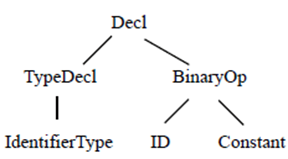
\includegraphics[scale=0.6]{ast_example.png}
\caption{An example of program AST}
\label{AST_sample}
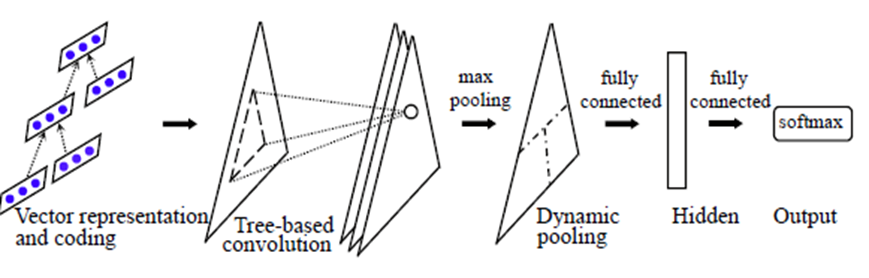
\includegraphics[scale=0.4]{tbcnn_struct.png}
\caption{A general structure of tree-based convolution neural network}
\label{tbcnn_struct}
\end{figure}

For programming languages we can build a tree representation (AST).
The AST for a small code snippet shown on a figure~\ref{AST_sample}.
Each node in the AST is an abstract component in program source code.
In the AST information about code structure store as parent/children relations.
A node represent as $p$ with children $c_1, \cdots, c_n$.
To work with AST nodes we need to represent them as vector with real values. 
Such vector representation named \textit{embedding}.



\subsection{Embeddings}
\begin{figure}
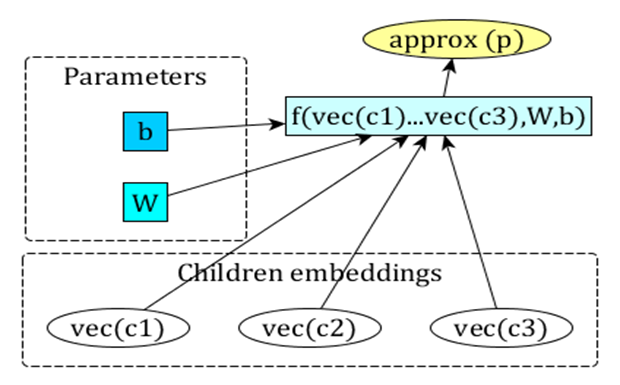
\includegraphics[scale=0.3]{children_approx.png}
\caption{A visualization of children approximation}
\label{child_approx}
\end{figure}
Every embedding capture information about type and relation information (position in tree) for it AST node.
During the embedding learning process we want similar vector representation (with a small distance) for nodes, that are often found in a similar context (i.e FOR and WHILE). To capture relation information we use children approximation (figure~\ref{child_approx}). 

Formally, let $\vect(\cdot) \in \mathbb{R}^{N_f}$ be
the feature representation of a node, where $N_f$ is the feature dimension.
For each non-leaf node $p$ and its direct children $c_1, \cdots, c_n$, we would like
\begin{equation}
\vect(p) \approx \tanh\left(\sum\nolimits_i l_iW_{\text{code},i}\cdot \vect(c_i) + \bm b_{\text{code}}\right)
\label{eCode}
\end{equation}
\noindent where $W_{\text{code},i}\in\mathbb{R}^{N_f\times N_f}$ is the weight
matrix corresponding to the node $c_i$; $\bm b_{\text{code}}\in \mathbb{R}^{N_f}$ is the bias.
$l_i = \frac{\#\text{leaves under } c_i}{\#\text{leaves under } p}$ is the coefficient of the weight.
(Weights $W_{\text{code},i}$ are weighted by leaf numbers.)





\subsection{Combination layer}
\begin{figure}
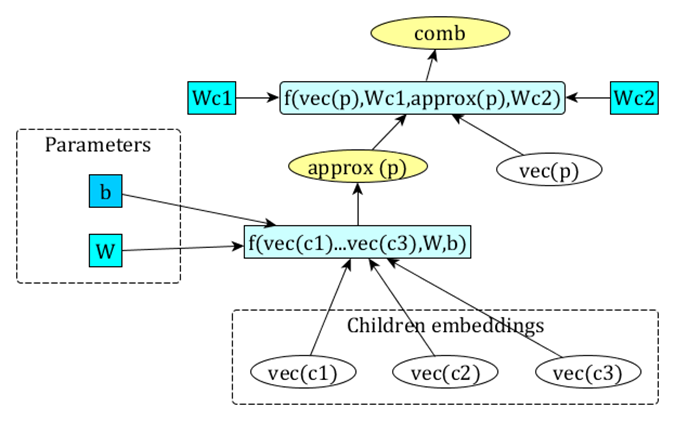
\includegraphics[scale=0.3]{combination.png}
\caption{A visualization of embeddings and children approximation combination}
\label{combination}
\end{figure}
After we trained embeddings for every AST node, we would like to feed them to a convolution layer. For leaf
node we use learned representation, but for non-leaf nodes we want to use a combination of trained embedding
and children approximation (figure~\ref{combination}).
Formally let $c_1, \cdots, c_n$ be the children of node $p$ and the combined vector for this node
is $\bm p$. We have
\begin{align}
\nonumber
\bm p &= W_{\text{comb1}}\cdot \vect(p)\\ \nonumber
 &+ W_{\text{comb2}}\cdot
\tanh\left(\sum\nolimits_{i} l_iW_{\text{code},i}\cdot\vect(x_i)+\bm b_{\text{code}}\right)
\end{align}
where $W_{\text{comb1}}, W_{\text{comb2}}\in\mathbb{R}^{N_f\times N_f}$ are the parameters
for combination. They are initialized as diagonal matrices and then fine-tuned during training.




\subsection{Convolution layer}
\begin{figure}
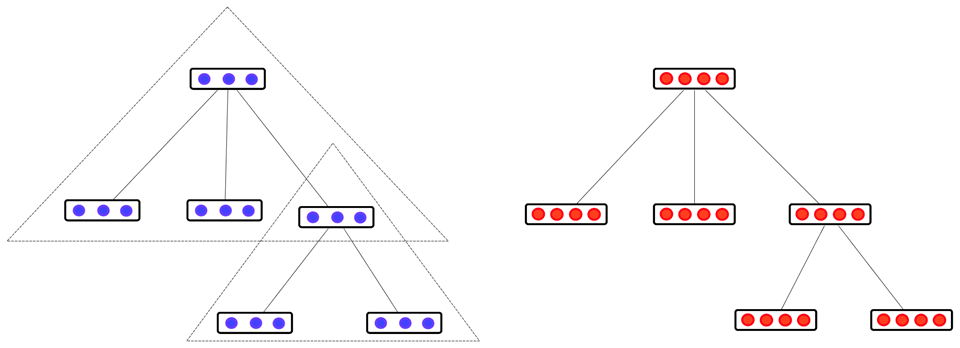
\includegraphics[scale=0.3]{conv_layer.png}
\caption{A visualization of convolution over tree structure}
\label{conv_layer}
\end{figure}
Now we have vector representation for each node in tree and now we apply convolution (figure~\ref{conv_layer}).
We applying convolution for each depth-1 subtree to extract features from every node relation group.
During convolution process we translate vectors for each node from embedding space to convolution space.

Formally the convolution process is:
\begin{equation}\nonumber
\bm y = \relu\left(\sum\nolimits_{i=1}^n W_{\text{conv},i}\cdot\bm x_i +\bm b_{\text{conv}}\right)
\end{equation}
where $\bm y, \bm b_{\text{conv}}\!\!\in\!\mathbb{R}^{N_c}$, $W_{\text{conv},i}\!\!\in\!\mathbb{R}^{N_c\times N_f}$. ($N_c$ is the number of feature detectors.)


\subsection{Pooling}
\begin{figure}
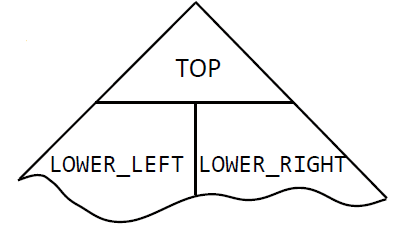
\includegraphics[scale=0.3]{three_way.png}
\caption{Subtrees (parts) of original tree}
\label{three_way}
\end{figure}

After convolution we have a new tree in a convolution space with extracted features.
The new tree has the same shape and size as the original one, which is varying among
different programs. So, the extracted features cannot be fed to a fixed-size neural layer.
Dynamic pooling \cite{dynamic} is applied to solve this problem.

The simplest approach is to pool all features to one vector. We call this
\textit{one-way pooling}. Concretely, the maximum value in each dimension is taken from the
features that are detected by tree-based convolution. In other words we pick a strongest detected feature. An alternative, is \textit{three-way pooling}, where features are pooled to 3 parts, TOP, LOWER\_LEFT,
and LOWER\_RIGHT, according to the their positions in the AST (figure~\ref{three_way}).


\subsection{Classifier}
We use vectors after pooling as classifier inputs to solve the problem of author identification.
Each one of three vectors contains information about author code style, structure and other things which neural network understood during training process. In out of classifier we have a one-hot encoded vector, represented an author from an original subset of authors.


\section{Evaluation}
At first we trained embeddings on a large dataset with Java 8 code. We confirm that learned vectors are respond 
to their definition (small distance for similar AST tokens).\\
Secondly we evaluate classifier on an open source repository from GitHub with 20 authors.
\subsection{Embeddings evaluation}
\begin{figure}
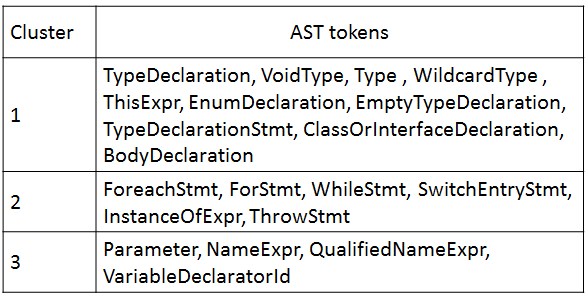
\includegraphics[scale=0.6]{embed_clust.png}
\caption{K-means clustering of embeddings}
\label{clusters}
\end{figure}

To evaluate quality of trained embeddings we apply K-means clustering to a subset of embeddings.
As shown at a result table (figure~\ref{clusters}) tokens which are corresponds to similar context have a 
quite similar vector representation.

\subsection{Classifier evaluation}
\begin{figure}
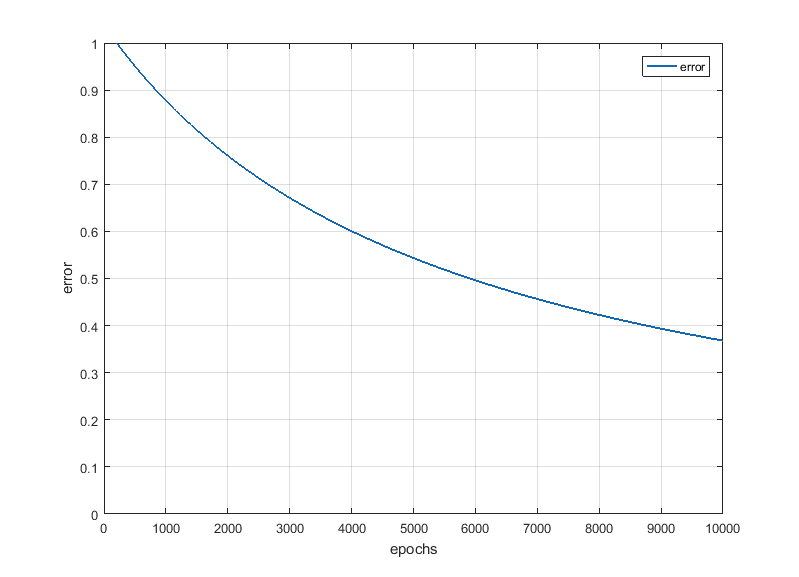
\includegraphics[scale=0.4]{test_err.png}
\caption{Error of author classification during training process}
\label{class_err}
\end{figure}

To evaluate quality of author classifier based on tree-based convolution we train TBCNN and classifier for 10000 epoch and measure an error of author identification (figure~\ref{class_err}). We use methods from target repository as dataset for our network. After many attempts we achieve about 60 percent accuracy  in author classification task.


\bibliography{}

\end{document}